% Content of Worksheet 02, shared by the problem sheet and the solution sheet.
% Solutions are wrapped in the `solution` environment and appear only when the
% driver defines \ipsshowsolutions.

\ipsmaketitle

This worksheet is ungraded practice, with the same shape and level as the final exam.
Plan up to 2 hours for a serious pass.
Work each problem through on paper before you open the solutions, and show your algebra:
the exam asks for the steps, not only the number.
Some parts state an intermediate result (``show that\,\ldots''); use it to check your work, and to continue if a step resists.
Carry at least four significant figures through the intermediate steps (the worked solutions print five) and round only at the end.

\begin{given}[Constants and data]
$1\ \mathrm{yr} = 3.156 \times 10^{7}\ \mathrm{s}$ \quad
$1\ \mathrm{d} = 86\,400\ \mathrm{s}$ \quad
$\Mearth = 5.972 \times 10^{24}\ \mathrm{kg}$ \quad
$\Rearth = 6371\ \mathrm{km}$ \quad
$R_{\mathrm{Moon}} = 1737\ \mathrm{km}$

\vskip4pt
Thermal diffusivity of rock $\kappa = 10^{-6}\ \mathrm{m^2\,s^{-1}}$ \quad
Age of the solar system $4.57$ Gyr \quad
Earth's core mass fraction $x = 0.32$ \quad
silicate heat capacity $c_p = 1250\ \mathrm{J\,kg^{-1}\,K^{-1}}$

\vskip6pt
\begin{tabular}{@{}lccc@{}}
\toprule
Isotope & Half-life (Gyr) & Heat production (W per kg isotope) & BSE concentration \\
\midrule
${}^{238}\mathrm{U}$  & $4.47$  & $9.5 \times 10^{-5}$ & $20\ \mathrm{ppb}$ \\
${}^{235}\mathrm{U}$  & $0.704$ & $5.7 \times 10^{-4}$ & $0.14\ \mathrm{ppb}$ \\
${}^{232}\mathrm{Th}$ & $14.0$  & $2.6 \times 10^{-5}$ & $80\ \mathrm{ppb}$ \\
${}^{40}\mathrm{K}$   & $1.25$  & $2.9 \times 10^{-5}$ & $28\ \mathrm{ppb}$ \\
\bottomrule
\end{tabular}

\vskip4pt
{\footnotesize Isotope table as in the Lecture~3 notes (BSE = bulk silicate Earth; $1\ \mathrm{ppb} = 10^{-9}$ by mass).
Hf-W constants as in the Lecture~4 notes: $\mathcal{Q}_\mathrm{W} = 10^4$,
$({}^{182}\mathrm{Hf}/{}^{180}\mathrm{Hf})_0 = 1.02 \times 10^{-4}$,
$\lambda = 7.79 \times 10^{-2}\ \mathrm{Myr^{-1}}$ ($t_{1/2} = 8.9$ Myr).}
\end{given}


% ════════════════════════════════════════════════════════════
\problem{The radiogenic clock}

Radioactive decay powers planetary interiors on two very different timescales.
Here you compute the long-lived budget from the isotope table, then place both timescales in the planetary context.

\parti The isotope table refers to the bulk silicate Earth (BSE): the mantle plus crust, without the core.
Compute the BSE mass from $\Mearth$ and the core mass fraction $x$, then compute the present-day
specific heating rate of BSE rock by summing the four isotopes
(show that it is $4.872 \times 10^{-12}\ \mathrm{W\,kg^{-1}}$).
Round $M_\mathrm{BSE}$ to one significant figure, give Earth's present radiogenic power in TW
and compare it with the value quoted in the notes.

\begin{solution}
The BSE mass is the non-core fraction of Earth's mass:
\[
  M_\mathrm{BSE} = (1 - 0.32) \times 5.972 \times 10^{24} = 4.0610 \times 10^{24}\ \mathrm{kg}.
\]
Each isotope contributes (concentration) $\times$ (heat production per kg of isotope):
\[
  {}^{238}\mathrm{U}:\ 20 \times 10^{-9} \times 9.5 \times 10^{-5} = 1.9000 \times 10^{-12}\ \mathrm{W\,kg^{-1}},
\]
\[
  {}^{235}\mathrm{U}:\ 0.14 \times 10^{-9} \times 5.7 \times 10^{-4} = 7.9800 \times 10^{-14},
  \quad
  {}^{232}\mathrm{Th}:\ 80 \times 10^{-9} \times 2.6 \times 10^{-5} = 2.0800 \times 10^{-12},
\]
\[
  {}^{40}\mathrm{K}:\ 28 \times 10^{-9} \times 2.9 \times 10^{-5} = 8.1200 \times 10^{-13}.
\]
The sum is
\[
  h_\mathrm{today} = (1.9000 + 0.0798 + 2.0800 + 0.8120) \times 10^{-12}
                   = 4.8718 \times 10^{-12}\ \mathrm{W\,kg^{-1}},
\]
which matches the printed checkpoint. With the round BSE mass:
\[
  P_\mathrm{today} = 4.872 \times 10^{-12} \times 4.0 \times 10^{24} = 1.9488 \times 10^{13}\ \mathrm{W} \approx 19.5\ \mathrm{TW}.
\]
\answer{$P_\mathrm{today} \approx 19.5$ TW, consistent with the 19--20 TW quoted in the Lecture~3 notes.}
\end{solution}

\parti The radiogenic-heating figure in the Lecture~3 notes shows the short-lived isotope
${}^{26}\mathrm{Al}$ ($t_{1/2} = 0.72$ Myr) crossing below the summed long-lived curve.
Read off the approximate crossover time from the figure.
How many ${}^{26}\mathrm{Al}$ half-lives is that, and by what factor has
${}^{26}\mathrm{Al}$ decayed by then?

\begin{solution}
The dashed ${}^{26}\mathrm{Al}$ curve crosses the solid long-lived total at roughly $10$ Myr after CAI formation.
That is
\[
  \frac{10\ \mathrm{Myr}}{0.72\ \mathrm{Myr}} = 13.9 \approx 14\ \text{half-lives},
\]
so the isotope has decayed by
\[
  2^{13.9} = 1.5 \times 10^{4}.
\]
\answer{Crossover near $10$ Myr, about 14 half-lives, a decline by a factor $\sim 1.5 \times 10^4$: short-lived heating is a property of the first few Myr only.}
\end{solution}

\parti In 2 to 3 sentences: why do U, Th, and K reside in the mantle and crust rather than in
the core, and what does this imply for \emph{where} radiogenic heat is released inside Earth?

\begin{solution}
U, Th, and K are lithophile in the Goldschmidt classification: during metal-silicate
separation they stay in the silicate phase rather than following the iron into the core.
As incompatible elements they are further concentrated into the last-crystallising liquids,
and so into the crust. Radiogenic heat is therefore released in the silicate shell,
roughly half of it in the thin crust, and essentially none inside the core, whose heat
budget is set by cooling and crystallisation instead.
\answer{Lithophile behaviour keeps the heat producers in the silicate shell; the core receives essentially no radiogenic heating.}
\end{solution}


% ════════════════════════════════════════════════════════════
\problem{Conduction fails, convection takes over}

Whether a body can cool by conduction alone is a question of size.
Here you find the size limit, then show that Earth's mantle convects instead, and how vigorously.

\parti Compute the conductive cooling timescale $\tau = L^2/\kappa$ for the Moon, using
$L = R_\mathrm{Moon}$, and compare with the
age of the solar system. Then invert the timescale: what is the largest body size that
\emph{can} cool conductively within $4.57$ Gyr?

\begin{solution}
\[
  L^2 = (1.737 \times 10^{6})^2 = 3.0172 \times 10^{12}\ \mathrm{m^2},
  \qquad
  \tau = \frac{3.0172 \times 10^{12}}{10^{-6}} = 3.0172 \times 10^{18}\ \mathrm{s}.
\]
In years:
\[
  \tau = \frac{3.0172 \times 10^{18}}{3.156 \times 10^{7}} = 9.5602 \times 10^{10}\ \mathrm{yr},
\]
about 21 times the age of the solar system, so even the Moon cannot
have cooled through its full radius by conduction alone. Inverting, with the age in seconds
$t = 4.57 \times 10^{9} \times 3.156 \times 10^{7} = 1.4423 \times 10^{17}$ s:
\[
  L = \sqrt{\kappa\,t} = \sqrt{10^{-6} \times 1.4423 \times 10^{17}} = \sqrt{1.4423 \times 10^{11}}
    = 3.798 \times 10^{5}\ \mathrm{m} \approx 380\ \mathrm{km}.
\]
\answer{$\tau \approx 9.6 \times 10^{10}$ yr $\gg$ 4.57 Gyr; only bodies below $\approx 380$ km cool conductively, larger ones must convect, or stay hot.}
\end{solution}

\parti Compute the Rayleigh number of Earth's mantle,
\[
  \mathrm{Ra} = \frac{\alpha\,\rho\,g\,\Delta T\,d^3}{\kappa\,\eta},
\]
with $\alpha = 2 \times 10^{-5}\ \mathrm{K^{-1}}$, $\rho = 4000\ \mathrm{kg\,m^{-3}}$,
$g = 10\ \mathrm{m\,s^{-2}}$, $\Delta T = 2500\ \mathrm{K}$, mantle depth $d = 3000$ km, and
dynamic viscosity $\eta = 10^{21}$ Pa\,s.
Compare with the critical value $\mathrm{Ra}_c \approx 1708$.

\begin{solution}
Numerator first:
\[
  \alpha\,\rho\,g\,\Delta T = 2 \times 10^{-5} \times 4000 \times 10 \times 2500 = 2000\ \mathrm{kg\,m^{-3}\,s^{-2}},
  \qquad
  d^3 = (3 \times 10^{6})^3 = 2.7 \times 10^{19}\ \mathrm{m^3},
\]
so the numerator is $2000 \times 2.7 \times 10^{19} = 5.4 \times 10^{22}$. The denominator:
\[
  \kappa\,\eta = 10^{-6} \times 10^{21} = 10^{15}.
\]
Therefore
\[
  \mathrm{Ra} = \frac{5.4 \times 10^{22}}{10^{15}} = 5.4 \times 10^{7},
\]
and
\[
  \frac{\mathrm{Ra}}{\mathrm{Ra}_c} = \frac{5.4 \times 10^{7}}{1708} = 3.162 \times 10^{4}.
\]
\answer{$\mathrm{Ra} \approx 5.4 \times 10^{7}$, over $3 \times 10^4$ times critical: the mantle convects vigorously despite its enormous viscosity.}
\end{solution}

\parti Judge this claim in 2 to 3 sentences:
\emph{``Doubling the mantle's temperature contrast $\Delta T$ would double the convective heat flux.''}

\begin{solution}
False. The convective flux is $q \propto \mathrm{Nu} \times \Delta T$, where the Nusselt
number Nu (the factor by which convection beats conduction) scales as
$\mathrm{Ra}^{1/3} \propto \Delta T^{1/3}$, so
$q \propto \Delta T^{4/3}$: doubling $\Delta T$ raises the flux by
$2^{4/3} = 2.52$, more than double. A hotter mantle does not just carry more heat per
parcel, it also convects more vigorously.
\answer{False: $q \propto \Delta T^{4/3}$, so the flux rises by a factor $2.52$.}
\end{solution}


% ════════════════════════════════════════════════════════════
\problem{A minimal thermal evolution model}

The heat budget of the Lecture~3 notes (radiogenic heating in, convective heat loss out) can be
turned into a one-line model of Earth's thermal history. This problem assembles the model on
paper and then reads Earth's thermal history from its numerical solution.

\parti Problem 2(c) already used the scaling $q \propto \Delta T^{4/3}$; derive it now in one
line from $\mathrm{Nu} \propto \mathrm{Ra}^{1/3}$ and $\mathrm{Ra} \propto \Delta T$ (all other
parameters fixed). Writing $T$ for the mantle temperature contrast, energy
conservation for the silicate shell then reads
\[
  C\,\frac{\mathrm{d}T}{\mathrm{d}t} = H(t) - Q(T),
  \qquad
  Q(T) = Q_0 \left(\frac{T}{T_0}\right)^{4/3},
  \qquad
  H(t) = H_\mathrm{f}\,e^{-t/\tau_r},
\]
with $C = M_\mathrm{BSE}\,c_p$ the heat capacity of the silicate shell.
State in one sentence each what the two right-hand terms represent.

\begin{solution}
The conductive flux across the layer is $q_\mathrm{cond} \propto \Delta T$, and convection
multiplies it by Nu:
\[
  Q \propto \mathrm{Nu} \times \Delta T \propto \Delta T^{1/3} \times \Delta T = \Delta T^{4/3}.
\]
$H(t)$ is the radiogenic heat input, a single exponential standing in for the summed decay
of the four long-lived isotopes; $Q(T)$ is the convective heat loss through the surface,
rising steeply with mantle temperature. The balance of the two drives $\mathrm{d}T/\mathrm{d}t$.
\answer{$Q \propto \Delta T^{4/3}$; heating in, parametrised convective cooling out.}
\end{solution}

\parti The figure shows the numerical solution of the model, integrated from
$T(0) = 3000$ K over 4.5 Gyr with $H_\mathrm{f} = 94$ TW, $\tau_r = 2.91$ Gyr,
$Q_0 = 47$ TW at $T_0 = 2500$ K, and
$C = 4.0 \times 10^{24} \times 1250 = 5.0 \times 10^{27}\ \mathrm{J\,K^{-1}}$.

\begin{center}
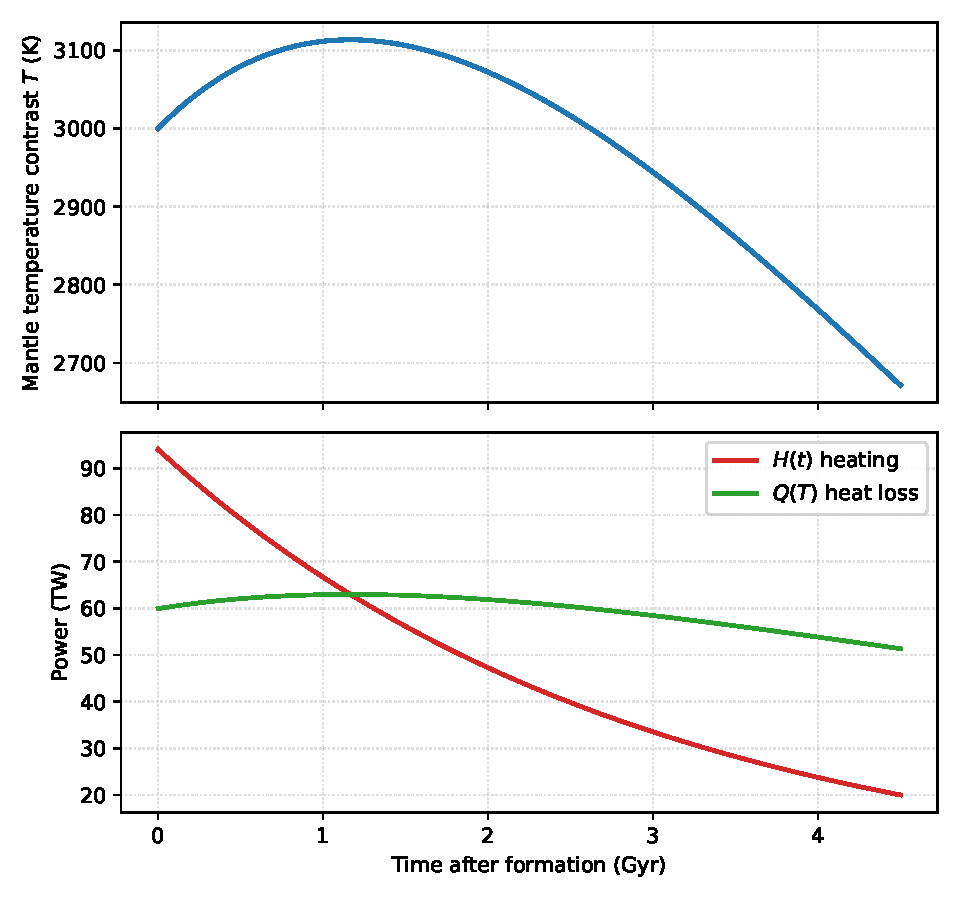
\includegraphics[width=0.72\linewidth]{figures/thermal_evolution_solution}
\end{center}

Read off: the maximum temperature and when it occurs, the final temperature
$T(4.5\ \mathrm{Gyr})$, and the final Urey ratio $H/Q$.
Then explain in one or two sentences why the temperature first \emph{rises} although the
heat source only decays.

\begin{solution}
The temperature curve peaks at $T \approx 3110$ K at $t \approx 1.2$ Gyr and ends at
$T(4.5\ \mathrm{Gyr}) \approx 2670$ K. At 4.5 Gyr the two power curves read
$H \approx 20$ TW and $Q \approx 51$ TW, so the final Urey ratio is
$H/Q \approx 20/51 \approx 0.39$.
The curve first rises because at 3000 K the convective loss ($\approx 60$ TW) is smaller than
the initial heating (94 TW): the interior warms until $Q$ catches up with $H$; from
$\sim$1.2 Gyr onward the planet tracks the decaying heat source downward, cooling ever after.
\answer{Peak $\approx 3110$ K at $\approx 1.2$ Gyr; $T(4.5) \approx 2670$ K; Urey ratio $\approx 0.39$. Early self-heating, then long secular cooling.}
\end{solution}

\parti Set $H = 0$ in the model and solve it analytically: show that at late times the
temperature falls off as $T \propto t^{-3}$.
What does this limit say about how quickly a small, radiogenically dead body fades?

\begin{solution}
With $H = 0$,
\[
  C\,\frac{\mathrm{d}T}{\mathrm{d}t} = -\frac{Q_0}{T_0^{4/3}}\,T^{4/3}.
\]
Separate variables:
\[
  T^{-4/3}\,\mathrm{d}T = -\frac{Q_0}{C\,T_0^{4/3}}\,\mathrm{d}t
  \quad\Rightarrow\quad
  -3\,T^{-1/3} = -\frac{Q_0}{C\,T_0^{4/3}}\,t + \mathrm{const},
\]
so $T^{-1/3}$ grows linearly with $t$, and at late times
\[
  T \propto t^{-3}.
\]
A body without radiogenic heating cools fast at first (the $T^{4/3}$ loss is strong while
it is hot) but fades on a long power-law tail rather than exponentially: cooling slows as the
driving contrast collapses.
\answer{$T \propto t^{-3}$: fast early cooling, then a slow power-law fade.}
\end{solution}


% ════════════════════════════════════════════════════════════
\problem{Building a core and dating it}

Core formation is fast, chemically selective, and datable.
Here you predict what it leaves behind in the mantle, and read the isotopic clock it starts.

\parti Let $x$ be the core mass fraction and $D = C^\mathrm{metal}/C^\mathrm{silicate}$ the
metal-silicate partition coefficient of a trace element. Assuming the whole planet
equilibrated once, show from mass conservation that the mantle retains a fraction
\[
  \frac{C^\mathrm{silicate}}{C^\mathrm{bulk}} = \frac{1}{1 + x\,(D - 1)}
\]
of the bulk concentration. Evaluate it for iridium with $D = 10^{4}$ and $x = 0.32$.

\begin{solution}
Per unit planet mass, the element is conserved:
\[
  C^\mathrm{bulk} = x\,C^\mathrm{metal} + (1 - x)\,C^\mathrm{silicate}
                  = C^\mathrm{silicate}\,\left[x D + (1 - x)\right]
                  = C^\mathrm{silicate}\,\left[1 + x(D - 1)\right],
\]
using $C^\mathrm{metal} = D\,C^\mathrm{silicate}$. Inverting gives the stated fraction. For iridium:
\[
  x(D - 1) = 0.32 \times 9999 = 3199.7,
  \qquad
  \frac{C^\mathrm{silicate}}{C^\mathrm{bulk}} = \frac{1}{3200.7} = 3.124 \times 10^{-4}.
\]
\answer{The mantle should retain only $\approx 3.1 \times 10^{-4}$ of its bulk iridium; with the larger $D$ values in the notes' range ($10^4$--$10^6$) the predicted remainder is smaller still.}
\end{solution}

\parti The observed iridium depletion of Earth's mantle is a factor $\sim 1000$, i.e.\ the
mantle retains $\sim 10^{-3}$ of chondritic. Compare with your prediction from part (a) and
explain, in 2 to 3 sentences, what the discrepancy implies. What single observation about the
element \emph{ratios} clinches the interpretation?

\begin{solution}
The mantle holds at least 3 times more iridium than one-stage equilibration predicts
(and orders of magnitude more for the higher $D$ values in the notes' range).
The standard resolution is the late veneer: after core formation ended, Earth accreted a
final $\sim 0.5\%$ of its mass in chondritic material whose siderophile elements stayed in
the mantle, because no sinking metal remained to extract them. The clinching observation is
that the highly siderophile elements sit in \emph{chondritic proportions} to one another:
core extraction would have fractionated them (their $D$ values differ), whereas a late
chondritic addition preserves the ratios.
\answer{The excess records a late veneer of $\sim 0.5\%$ Earth masses of chondritic material after core formation; the unfractionated (chondritic) element ratios are the fingerprint.}
\end{solution}

\parti A planetesimal's mantle shows a tungsten excess $\varepsilon^{182}\mathrm{W} = +20$
with an Hf/W enrichment factor $(\mathrm{Hf}/\mathrm{W})/(\mathrm{Hf}/\mathrm{W})_\mathrm{CHUR} = 26$,
so the bracketed factor in the notes' two-stage equation is 25. Using the Hf-W constants from
the data box, show that $e^{-\lambda t_c} = 0.784$ and find the two-stage core-formation age
$t_c$. Compare with the accretion-timeline figure in the Lecture~4 notes.

\begin{solution}
The two-stage equation rearranges to
\[
  e^{-\lambda t_c} = \frac{\varepsilon^{182}\mathrm{W}}{\mathcal{Q}_\mathrm{W} \times 25 \times ({}^{182}\mathrm{Hf}/{}^{180}\mathrm{Hf})_0}
  = \frac{20}{10^{4} \times 25 \times 1.02 \times 10^{-4}}
  = \frac{20}{25.5} = 0.784,
\]
the printed checkpoint. Solving for $t_c$:
\[
  t_c = -\frac{\ln 0.784}{\lambda} = \frac{0.24335}{7.79 \times 10^{-2}} = 3.1238 \approx 3.1\ \mathrm{Myr}.
\]
This sits squarely in the planetesimal band of the accretion-timeline figure, which shows
planetesimal cores differentiating within the first few Myr, well before the planets finish
growing.
\answer{$t_c \approx 3.1$ Myr: this body formed its core in the planetesimal era.}
\end{solution}

\parti In 2 to 3 sentences: why can the Hf-W chronometer not date any core-forming event
later than roughly 45 Myr after CAIs, and what tool takes over for such late events?

\begin{solution}
Beyond $\sim$5 half-lives ($\approx 45$ Myr) the parent ${}^{182}\mathrm{Hf}$ is effectively
extinct: whatever ${}^{182}\mathrm{W}$ exists is already made and distributed, so a later
core extraction changes nothing in the mantle's $\varepsilon^{182}\mathrm{W}$ and the clock
reads nothing. Late events (such as the nucleation of Earth's inner core, billions of years
after formation) are instead constrained by thermal-evolution modelling, as in the notes.
\answer{After $\sim$45 Myr the parent isotope is extinct and the chronometer is blind; thermal-evolution modelling takes over.}
\end{solution}


% ════════════════════════════════════════════════════════════
\problem{Dynamos and shields}

A convecting metallic core can maintain a magnetic field, and that field carves a cavity in
the solar wind. Here you test both, for two very different bodies.

\parti Start from pressure balance at the dayside magnetopause,
$\tfrac{1}{2}\rho_\mathrm{sw} v_\mathrm{sw}^2 = B_\mathrm{mp}^2/(2\mu_0)$, with a dipole
field $B(r) = B_0\,(R_p/r)^3$. Show that the standoff distance obeys
\[
  r_\mathrm{mp} = R_p \left(\frac{B_0^{2}}{\mu_0\,\rho_\mathrm{sw} v_\mathrm{sw}^{2}}\right)^{1/6}.
\]
During a coronal mass ejection the solar-wind density rises tenfold at fixed speed.
Starting from Earth's typical $r_\mathrm{mp} = 10\,R_\oplus$, compute the new standoff
distance.

\begin{solution}
Insert the dipole law at $r = r_\mathrm{mp}$ into the pressure balance:
\[
  \frac{1}{2}\rho_\mathrm{sw} v_\mathrm{sw}^2 = \frac{B_0^2\,(R_p/r_\mathrm{mp})^6}{2\mu_0}
  \quad\Rightarrow\quad
  \left(\frac{r_\mathrm{mp}}{R_p}\right)^{6} = \frac{B_0^{2}}{\mu_0\,\rho_\mathrm{sw} v_\mathrm{sw}^{2}},
\]
which is the stated result after taking the sixth root. The standoff therefore scales as
$\rho_\mathrm{sw}^{-1/6}$ at fixed $B_0$ and $v_\mathrm{sw}$:
\[
  r_\mathrm{mp}' = 10\,R_\oplus \times 10^{-1/6} = \frac{10}{1.4678}\,R_\oplus = 6.813\,R_\oplus \approx 6.8\,R_\oplus.
\]
\answer{$r_\mathrm{mp} \propto (B_0^2/\rho_\mathrm{sw} v_\mathrm{sw}^2)^{1/6}$; a tenfold density surge compresses Earth's magnetopause from $10$ to $\approx 6.8\,R_\oplus$. The sixth root is why the magnetosphere is so stable against solar-wind buffeting.}
\end{solution}

\parti Ganymede's dynamo operates in a liquid iron shell of thickness $L \approx 300$ km
with magnetic diffusivity $\eta = 1\ \mathrm{m^2\,s^{-1}}$. If its convection stopped, the
field would decay ohmically on the timescale
$\tau_\mathrm{ohm} = L^2/\eta \approx 3 \times 10^{3}$ yr (verify this in one line if you
wish). Explain in 2 to 3 sentences what this timescale, set against the age of the solar
system, proves about the field the Galileo spacecraft measured in 1996, and why a
``fossil field'' interpretation fails.

\begin{solution}
The one-line check: $\tau_\mathrm{ohm} = (3.0 \times 10^{5})^2 / 1 = 9.0 \times 10^{10}$ s
$= 9.0 \times 10^{10} / 3.156 \times 10^{7} = 2852$ yr.
Against 4.57 Gyr this is an instant: any field created in Ganymede's past would have
decayed away millions of times over. A fossil field therefore cannot survive; the field
Galileo measured must be regenerated continuously, so the 1996 detection is direct proof of
a dynamo operating \emph{now}.
\answer{$\tau_\mathrm{ohm} \approx 3 \times 10^{3}$ yr $\lll$ 4.57 Gyr: no fossil field survives, so the measured field proves a currently running dynamo.}
\end{solution}

\parti Judge this claim in 2 to 3 sentences:
\emph{``Venus has no magnetic field because it rotates too slowly.''}

\begin{solution}
Not supported. Numerical dynamo simulations show that slow rotation alone does not prevent
dynamo action, and the scaling laws for field strength are essentially independent of
rotation rate. The likely culprits are the absence of a crystallising inner core (no
compositional buoyancy) and Venus's stagnant lid, which insulates the core and throttles the
convective power available to a dynamo; rotation is at most a secondary factor.
\answer{False as stated: the field is starved of convective power, not of rotation.}
\end{solution}
